% last updated in April 2002 by Antje Endemann
% Based on CVPR 07 and LNCS, with modifications by DAF, AZ and elle, 2008 and AA, 2010, and CC, 2011

\documentclass[runningheads]{llncs}
\usepackage{graphicx}
\usepackage{amsmath,amssymb} % define this before the line numbering.
\usepackage{ruler}
\usepackage{color}
\usepackage{subfigure}
\usepackage[width=122mm,left=12mm,paperwidth=146mm,height=193mm,top=12mm,paperheight=217mm]{geometry}
\begin{document}
% \renewcommand\thelinenumber{\color[rgb]{0.2,0.5,0.8}\normalfont\sffamily\scriptsize\arabic{linenumber}\color[rgb]{0,0,0}}
% \renewcommand\makeLineNumber {\hss\thelinenumber\ \hspace{6mm} \rlap{\hskip\textwidth\ \hspace{6.5mm}\thelinenumber}}
% \linenumbers
\pagestyle{headings}
\mainmatter
\def\ECCV12SubNumber{295}  % Insert your submission number here

\title{Mimicry Evaluation and Identity Blending with Morph Space PCA} % Replace with your title

\titlerunning{ECCV-12 submission ID \ECCV12SubNumber}

\authorrunning{ECCV-12 submission ID \ECCV12SubNumber}

\author{Anonymous ECCV submission}
\institute{Paper ID \ECCV12SubNumber}


\maketitle

\begin{abstract}
The skill of expression mimicry must be learned without direct performance feedback\cite{grossberg2010children}, and study of this phenomenon would benefit from a metric characterising quality of imitation. We describe a face modelling tool allowing image representation in a high-dimensional morph space, compression to a small number of coefficients using PCA\cite{jolliffe2002principal}, and expression transfer between face models by projection of the source morph description into the target morph space. This technique allows statistical evaluation of mimicry quality and creation of an identity-blended avatar model whose high degree of realism suggests diverse applications in psychophysics, animation and affective computing.
\end{abstract}


\section{Introduction}


Expression mimicry is a key part of social interaction\cite{bavelas2007face} and communication strategy learning\cite{oberman2007face}. Unconscious imitation can reinforce feelings of affiliation and empathy between people\cite{lakin2003using}. How we learn to solve the correspondence problem of imitation, to replicate the movement of others without requiring a mirror to reveal our own facial action, is an open question\cite{grossberg2010children,sheppard1959evolution}.  Mimicry links the domains of visual perception, neural coding and translation of internal representations into motor commands.  It is often ascribed to mirror neurons\cite{rizzolatti2004mirror}, which fire during the performance and perception of an action, but such neurons are best considered as components of the process. There is currently a lack of broader computational models implementing mimicry\cite{dinstein2008mirror}, and their development calls for a precise method of evaluating imitation accuracy in order to benchmark bio-inspired and computational strategies.


Here we present a series of techniques aimed at the computational implementation of expression imitation, the removal of personal identity by blending facial characteristics, and the measurement of mimicry accuracy in human subjects.
The face space formalism\cite{valentine2001face} has proved an intuitive and useful guess at the brain's internal representation of facial characteristics. The na\"{i}ve version\cite{turk1991face} applies principal component analysis directly to raw image data in image space, producing a new coordinate frame whose axes correspond to the directions of greatest variation in the original data.

The PCA technique can be extended, firstly by including morphological data describing faces' shape and secondly by modifying the representation of each face so that it is relative to a mean. A series of portrait photographs can thus be used to create a coordinate frame which efficiently expresses the variation present in the input set. For ease of usage we will simply call this frame face space, recognising the more generic use of this term elsewhere in the literature\cite{valentine2001face}.  When the input image set comprises diverse configurations of one person's face, the resulting PCA space is effectively a controllable model of that face.


In the study of the perception of dynamic facial expression it would be very valuable to be able to separate facial motion from facial shape by mapping the motion onto an average face. However generating an average dynamic avatar is non-trivial, requiring extensive software engineering efforts\cite{itti2003realistic,rajan2002realistic} which often suffer from the uncanny valley effect\cite{mori1970uncanny}.

One cannot simply average up multiple faces performing some action under instruction as the timing of the behaviour may differ radically between people, leading to temporal misalignment and temporal blur. We have developed a novel method to circumvent this problem. First we build individual expression spaces for multiple actors. We then project frames from a sequence into the multiple expression spaces and average over the result. The sequence of averages is then processed by PCA to provide a photorealistic mean expression space.


\section{PCA Modelling of Morphed Faces}

This section describes in detail the pre-processing and PCA operations necessary to transform a set of input images into a face model.

We begin with a set of $n$ $h\times w$ input images $I_i$ showing facial portraits of one person effecting different expressions. One image is chosen as the reference image $I_r$. Each image $I_i$ is compared with the reference image using a gradient based motion estimation algorithm(the McGM\cite{mcowan1995algorithms,anderson2003real}) which produces, for each image, a full vector field (one vector per pixel) providing an estimate of the motion between the reference and target images. This is effectively a dense registration relation between $I_r$ and each $I_i$. A vector from a point on $I_r$ shows the new location of that point on $I_i$, and we refer to one such set of vectors as a warp field.

Each remaining image is represented by its difference from the reference image. $I_r$ should show a neutral expression, with the eyes open and the mouth slightly open, showing the teeth and a small black area between them (so that the McGM can find a way to warp the reference image to reconstruct any dental or buccal features in the remaining images).

The multichannel gradient model (McGM\cite{mcowan1995algorithms,anderson2003real}) is a bio-inspired algorithm which calculates a basis set of spatio-temporal derivatives by convolving the image sequence with derivative of Gaussian filters, and then combines them to form derivatives of the Taylor expansion in space and time. Ratios of the resulting terms then yield robust estimates of image motion between the reference image and each additional frame. In practice, each pair ($I_r$ and one $I_i$) are converted to greyscale and subsampled at several different resolutions before submission to the McGM. The resulting lower-resolution warp fields are combined into one field of the same size as $I_i$, which gives better results than single-scale motion analysis. 

In practice it is useful to constrain the input to some degree. Rigid head movement (translation or rotation) should be kept to a minimum, either by recording protocol or image registration by face detection (good results have been obtained with the commercially available toolkit FaceAPI\cite{website:fermentas-lambda}), so that the warp fields represent primarily changes in expression and not head movement. The background should be a uniform colour so that it does not contribute to the final model. Exposure and white balance should be kept constant during recording.
Once warp fields have been obtained for all images, the vectors at each pixel are averaged to give the mean warp field.



Each image $I_i$ is now expressed as two components (a similar dissociation to Blanz and Vetter's separation of 3D shape and texture\cite{blanz1999morphable}):
\begin{itemize}


\item Texture $T_i$: an image showing the textural component of the face shown in $I_i$. Anatomical points on textures are aligned with each other and with the mean face, as $T_i$ has been warped from $I_i$ to align it with the mean face.
\item Warp $W_i$: a warp field (full vector field the same size as $T_i$) showing how $T_i$ should be warped in order to realign it with the expression shown in $I_i$; see Fig. \ref{fig:subfigureExample1}\subref{fig:subfig3a}.
Operationally, the warp field is represented not by the relative displacement of each pixel (a true vector coding) but as the new position of each pixel (an absolute coding).
\end{itemize}


\begin{figure}[tb]
	\centering	\subfigure[One frame from a finished avatar.]{
	   	    \label{fig:subfig1a}
\includegraphics[height=3cm]{img/meanMorph.png}
	}	\hspace{0.5cm}\subfigure[The (rescaled) relative texture of an $I_i$.]{	   	    \label{fig:subfig2a}
	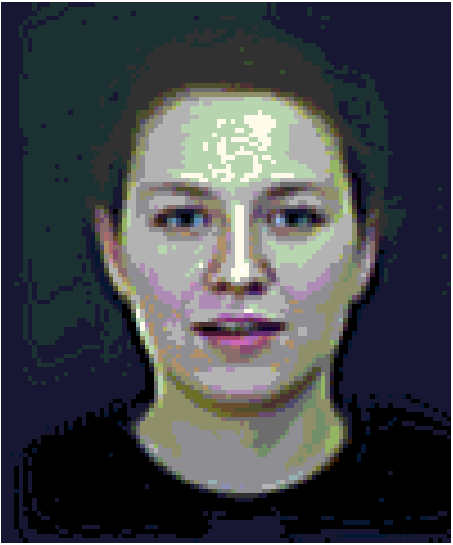
\includegraphics[height=3cm]{img/relTexture.png}
	}	\hspace{0.5cm}\subfigure[Quiver plot showing every 5th vector of a warp field.]{
	    	    \label{fig:subfig3a}
	    	    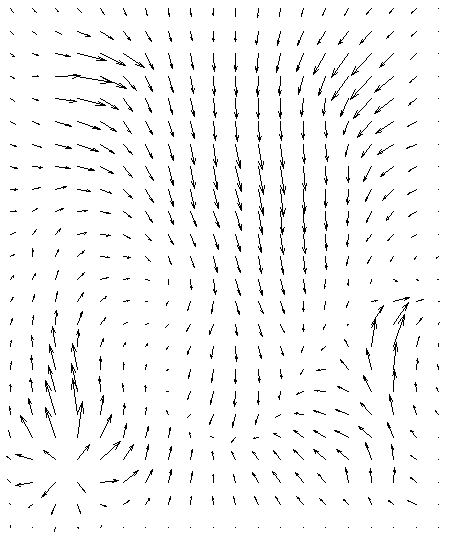
\includegraphics[height=3cm]{img/Warp.png}
	}
	
	\subfigure[Avatar generation. Each group shows a set of projected expressions; source faces are bordered in red. Centre bottom images show the morph average of each expression.]{
	   	    \label{fig:subfig4a}
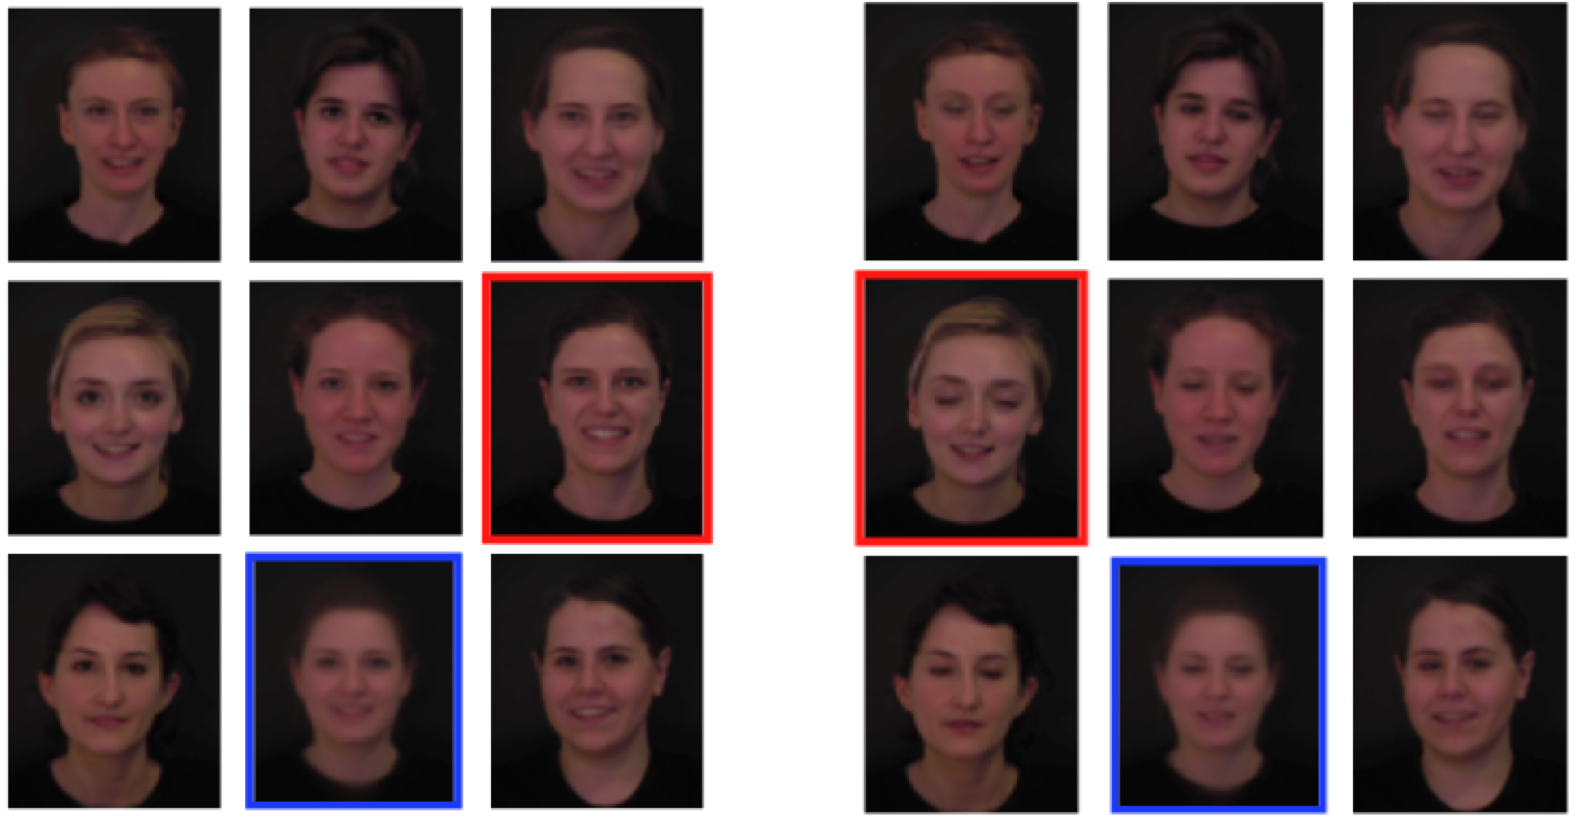
\includegraphics[scale=0.2]{img/fig2.png}
	}	\hspace{0.5cm}
	\caption{Components of a morph-modelled image and the avatar generation process.}
	\label{fig:subfigureExample1}
	\end{figure}




This representation decouples textural from configurational information, which is  useful. This means each can be be manipulated separately, as when the warp field is amplified to caricature an expression\cite{brennan1985caricature}.

Once each image $I_i$ has been represented as a morph pair  $\{T_i$,$W_i\}$, the data are nearly ready for principal component analysis. Two final preprocessing steps are performed: serialisation and mean relativisation.

As PCA operates on vectors of reals,  not more complex data structures, each morph tuple is serialised into a morph vector. This is done by iterating columnwise across the elements of the texture's colour channel matrices (R, G and then B), followed by the $x$ and $y$ warp field matrices, and  concatenating them into a vector.

The final vector is of length $w \times h \times (2 + 3)$, as each pixel in a $w \times h$ image is linked with 2 reals coding the $x$ and $y$ components of $W_i$ and 3 reals coding the RGB colour channels of $T_i$. A morph vector contains all the information necessary to reconstruct a face image, which is done by deserialising the vector, displacing the texture pixels by the warp field, and interpolating. This process is termed morphing (after the special effect\cite{rotshtein2004morphing}) and gives a very high-fidelity reconstruction of $I_i$.  The space of all possible morph vectors we refer to  as morph space, and it is a superset of that of all possible images (image space) as every image can be exactly represented in morph space by a texture with zero warp field.

We thus obtain $n$ morph vectors $M_i$. The mean morph $M_m$ is found and subtracted from each $M_i$, giving mean-relative morph vectors $R_i$. This operation models the assumption that identity changes are cognitively encoded in terms of difference from a stored mean, although this property would of course be implemented differently in the neural substrate than in the model's source code.
The relation $M_i = R_i + M_m$ splits each absolute morph vector (equivalent to a face image) into a constant part and a variable (relative) part. Fig. \ref{fig:subfigureExample1}\subref{fig:subfig2a} illustrates the texture component of an example relative morph vector.

The relative morph vectors $R_i$ are submitted directly to principal component analysis, which finds a new orthogonal coordinate frame such that, iteratively, each new axis encodes the maximum possible remaining variance in the data. We term the new frame a PCA space or expression space\footnote{Face and expression spaces are mathematically identical, but expression is constant in the former and identity is constant in the latter.}; dimensionality is normally between 50 and 100, which allows for very accurate image reconstruction while retaining a high degree of compression (for $200 \times 240$ images, morph space dimensionality is $200 \times 240 \times 5 = 240,000$, so a 100-d expression space has a compression factor of 2400).

Faces can now be expressed in terms of their coordinates in expression space, which is to say their loadings on the principal component axes. Passage from expression space to morph space is done by multiplying by a matrix encoding the embedding of the expression space reference frame in relative morph space, which we term the expression space matrix $P$. Reconstruction of an image from loadings $l$ involves

\begin{enumerate}
\item	Projection of expression space coordinates into relative morph space: $R = P \times l$, where $R$ is the relative morph space coordinate vector.
\item	Addition of the morph mean to generate absolute morph space coordinates $M = R + M_m$
\item	Image reconstruction by applying warp to texture and interpolating.
\end{enumerate}

A full PCA face model consists of the expression space matrix $P$, the morph mean $M_m$ and the variances of each principal component (used to generate faces in a realistic probability distribution).



\section{Expression Projection}

The twin decouplings of the morph space paradigm permit a very useful operation: the projection of an expression from one face model onto another. Consider two PCA models $A$ and $B$ generated from input images of two different people performing approximately the same sequence of expressions (or similar expressions in a different order).

 One might imagine that if facial morphologies are similar, the warp fields for each expression will be similar. If lighting conditions and skin tones are similar, the texture components will also be similar. Once mean warp fields and textures have been found and subtracted, similarity of the relative warps and textures depends only on similarity of actual expressions, not underlying facial attributes (which are subtracted by the relativisation process).
 
The principal components (in other words, the orientation of expression space in image space), however, are not guaranteed to be similar, as PCA may alter the sign and ordering of components\cite{jolliffe2002principal}. We therefore cannot rely on taking an image $I_a$ of person A, calculating its PC-loadings using $A$, and passing these loadings to model $B$, to reconstruct an image of person B exhibiting a similar expression. This process would rely on the two expression spaces being similarly oriented in common image space (they do not need to have close origins, since the correct morph mean for each model is subtracted and added in each case). In practice, axis signing and ordering may be different, and simply transferring the loadings does not always result in effective expression mimicry.

A more robust mimicry method is the following:

\begin{enumerate}


\item	Start with an image $I_a$ of person A, along with a PCA space $A$ for that individual and a PCA space $B$ for person B. We have the morph means $M_{ma}$ and $M_{mb}$.

\item	Encode $I_a$ as an absolute morph vector $M_a$ and then a relative morph vector $R_a$ with $ (R_a = M_a - M_{ma})$.
\item	Take the inner product of $R_a$ with the PCA matrix for person B ($P_b$). This gives a set of PC-loadings in person B's expression space $E_b$. We have
$L_b = R_a \times P_b$.

%TODO: insert that this is the inner product.
%CHange F to E everywhere.

This step in effect calculates the best possible representation of the variable component of $I_a$ (encoded by $R_a$) in $E_b$, the expression space for person B. Even if $E_b$ is very differently oriented from $E_a$, $R_a$ will still be sensibly reconstructable, even though its PC-loadings in $E_b$ may be very different than in $E_a$. The requirement that $E_a$ and $E_b$ be similarly oriented is thus removed.
\item	Generate a new relative morph vector $R_b$ by multiplying the calculated loadings $L_b$ by person B's PCA matrix:
$R_b = P_b \times L_b$.
This represents the reconstruction of $R_a$ (the variable component of $I_a$) in $E_b$.
\item	Add the mean morph vector $M_{mb}$ of person B. This represents combining the constant component of model B with the variable component transferred from $I_a$. We are in effect applying the expression of $I_a$ to the face of person B. We have $M_b = R_b + M_{mb}$.
\item	Reconstruct an image $I_b$ from $M_b$ by applying the warp component to the texture component and interpolating.


\end{enumerate}

This procedure is problematic when the source face is a very different shape from the target face, as projecting the source relative morph vector into the target PCA space will lead to an unnatural expression on the target (consider applying the warp of a smile exhibited on a wide, short face to a narrow, tall face). This mismatch can be avoided by transforming the warp and texture components of the morph vector before projection.

This is done by manually placing 3 keypoints on the morph mean images (which are generated during PCA modelling) for source and target identities, one at the centre of each eye and one at the centre of the philtrum. These define a triangle termed the faceframe. An affine transformation between source and target faceframes is defined and applied to the relative warp field and texture; this aligns them with the target faceframe, rendering it meaningful to add them to the target's morph mean. With 3 keypoints, only the eyes and philtrum are perfectly aligned, but the improvement is still substantial. 


\section{Avatar Generation}

The projection process, as it allows expressions to be replicated across different identities, enables another useful technique: the fusion of PCA models of several different people into one PCA model depicting an artificial identity. Conceptually and aesthetically, the physical characteristics of this new face are a blend of those of its ingredient faces. Mathematically, the new face is generated by morphing together ingredient faces.


The naive mathematical implementation of blending is finding the mean in a representational space. As Galton found\cite{galton1879composite}, this approach does not succeed if we average in image space, since not every point corresponds to an image. Direct averaging produces ghosted images which are textural but not anatomical hybrids. To generate sequences of realistic faces for mimicry animation we must therefore use morph space, in which many points in the subspace spanned by real data (input faces) correspond to anatomically plausible faces. Representing static images in morph space and finding the mean implements identity blending (like the classic morph special effect\cite{rotshtein2004morphing}) in static images. The same can be done for a PCA model by statically blending different expressions and then applying the PCA modelling procedure to the resulting images.


The following is a detailed description of our avatar generation process, as illustrated by Fig. \ref{fig:subfigureExample1}\subref{fig:subfig4a}.

\begin{enumerate}


\item	We begin with $k$ identities, each set $S^k$ containing $n^k$ portrait images of a particular person. These are subject to the same constraints on alignment and image characteristics as the single-identity PCA process described earlier.
\item	A reference image $r^k$ is chosen for each identity, subject to previously described constraints.
\item	A PCA model is generated for each identity, as described. Each  model brings with it a mean morph vector and an associated morph mean image.
\item	Each morph mean image is displayed and 3 keypoints are manually placed, one at the centre of each eye and one at the centre of the philtrum. These define a triangle termed the faceframe $f_i$.
\item Each input image $I^k_i$ is projected into $k-1$ other identities, producing $k$ copies of the same expression, which form the set $e^k_i$. During projection, the morph vector is affinely transformed to bring its faceframe into line with that of the target identity.
\item	Generated images are sharpened by convolving with an unsharp filter\cite{polesel2000image}.
\item	As images in the set $e^k_i$ have been projected into different faceframes, they are not aligned, and so a second transformation is performed (this time on image data only, as the generated images have no warp component). Each image in each $e^k_i$ can be transformed onto either \textit{a)} a reference faceframe $f_r$ (chosen arbitrarily from among the $k$ models) or \textit{b)} the faceframe corresponding to the source model for this expression ($f_k$).
\item	Once images in each $e^k_i$ have been aligned, they undergo the standard modelling process, but without the final step of PC analysis. In other words, they are each motion-compared with a reference image (we choose the projection onto the reference identity $I_r$); warp fields are generated and resourced to point from the mean warp; textures are reverse warped to align them onto the mean warp; fields and textures are assembled into morph vectors; and the mean morph vector is found. As each $e^k_i$ contains images of the same expression across multiple identities, the mean morph image will also exhibit that expression. Its identity, however, will have been morphed into a blend of the $k$ original identities.
\item The standard PCA modelling process is run on the set of blended images from each $e^k_i$; as this only happens once, a new reference image can be chosen in order to obtain the best warp fields. Alternatively, the reference image of the reference model can be used. We obtain a PCA model with a wide range of emotional diversity and a common blended identity. Its final appearance is illustrated in Fig. \ref{fig:subfigureExample1}\subref{fig:subfig1a}.

\end{enumerate}


%\begin{figure}[ht]
%	
%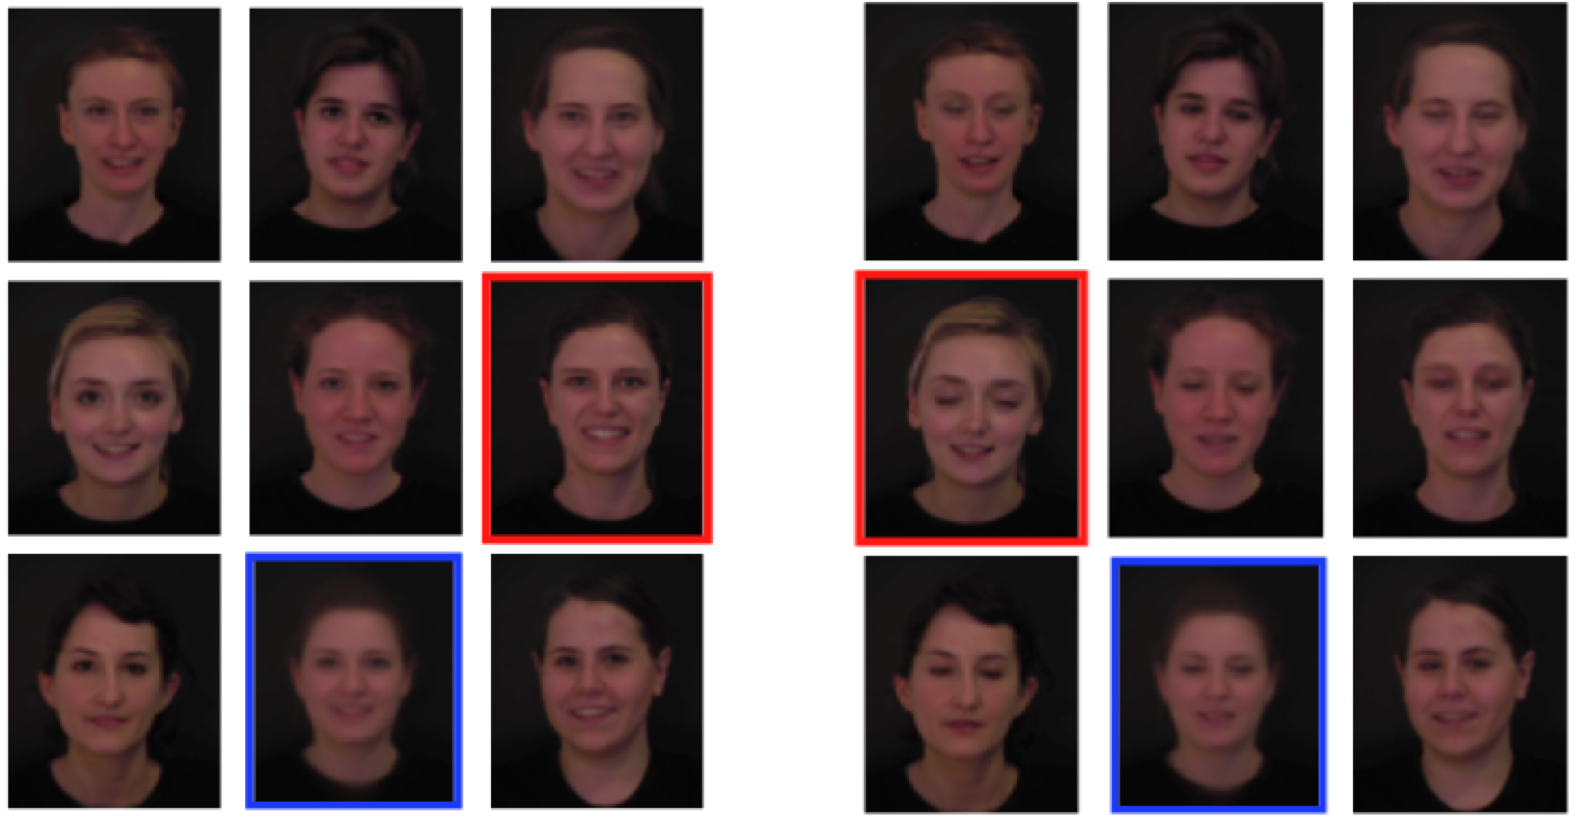
\includegraphics[scale=0.5]{img/fig2.png}
%\centering
%	\caption{Avatar generation. Top images show sets of projected expressions; source faces are bordered in red. Centre bottom images show the (unsharpened) morph average of each expression. Fig \ref{fig:subfigureExample1}\subref{fig:subfig1a} shows an example frame from the final avatar.}
%	\label{fig:subfigureExample}
%	\end{figure}

\section{Discussion}

We have described a PCA modelling process allowing compression of face images into a small number of expression space coordinates (principal component loadings), projection of expressions from one face model to another, and generation of an identity-blended avatar. These techniques have already been applied in\cite{berisha2010identifying,berisha2009photorealistic,cook2011exploring,griffin2011relative}.

%These techniques have already been applied to the identification of informationally significant face regions\cite{berisha2010identifying,berisha2009photorealistic} the investigation of adaptation to anti-expressions\cite{cook2011exploring} and the neural encoding of family resemblance\cite{griffin2011relative}. 


The avatar generation technique outlined is robust across diverse facial expressions and variations in facial morphology. Realism can be reduced, however, when the McGM is not able to accurately describe facial deformation by warp fields in the initial PCA stage (due to unsuitable illumination or non-smooth facial features such as glasses, piercings or facial hair) or where face shapes are different enough to make alignment difficult during the two transformation stages. As affine transforms are only done based on three keypoints, corresponding facial features will not always be brought into alignment. This is only a major problem if identities vary greatly in head size.

We envisage that future work could compensate for this problem by automatically defining more keypoints using commercially available face recognition software and transforming by arbitrary warping instead of affine transformation, as long as anatomical realism is maintained.
The addition of subexpression spaces which separately model individual features could allow constraints such as rigidity to be placed on specific features such as teeth and eyes. It would also allow comparison of the current (holistic) model with a local feature encoding scheme.

Computational mimicry has two main uses: generation of face stimuli which imitate others, and characterisation of real mimicry by subjects.
Given source morph vectors and a target PCA model, expressions can easily be projected from source to target. This can be done either for static faces or, by separately projecting each individual frame, for video sequences. Degrees of caricaturing can easily be applied. Such stimuli could form part of diverse psychophysical protocols, such as finding the detection threshold for erroneous mimicry or investigating to what extent caricaturing improves recognition. The ability to project expression means that it can be kept constant across identities, making it easier to investigate effects due to shape alone.

Natural mimicry can also be measured. Consider a protocol during which a subject is asked to mimic a portrait video sequence while a portrait recording is made. We can project the mimicry sequence from the subject into the PCA space of the stimulus, giving a sequence of PC loading vectors in the same expression space as the stimulus. This can be compared to the loading sequence of the mimicked video, either visually (by viewing the stimulus and its projection side-by-side) or using spatial distance measures or information theoretic measures such as mutual information or Shannon entropy. This would allow measurement of the distributed\cite{haxby2000distributed} face processing system's imitation accuracy.

The morph space PCA strategy is an intuitive, untrained way to measure mimicry in either human faces or artificial stimuli\cite{cook2012self}; it could also be used to benchmark other algorithms that perform imitation. The morph vector framework presents opportunities for extension such as the inclusion of local feature characteristics or high-level data concerning illumination or head direction.


The ability to generate a blended avatar renders it possible to generate realistic stimuli situated on the plausible side of the uncanny valley\cite{mori1970uncanny} (especially in terms of skin tone) but free from real-world identity. This avoids problems of privacy and ethics compliance (as the avatar is not a real person) and experimental bias (towards a particular identity). During the blending step, the output could be shifted away from the mean morph to change the appearance of the avatar, generating different identities for use in interactive software applications, games, or media.

The more source identities an avatar is built from, the more attractive the resulting PCA model will appear\cite{grammer1994human}. This could be leveraged in applications where positively-connotated faces can lend an advantage, such as animated user interface agents or virtual newsreaders\cite{muller2001face}.





\bibliographystyle{splncs}
\bibliography{egbib}





\end{document}
